\begin{mdframed}
    \textbf{La extensión máxima para esta sección es de 6 página.}
\end{mdframed}


\epigraph{``\textit{Non-reproducible single occurrences are of no significance to
science.}''}{---\citeauthor{popper2005logic},\citeyear{popper2005logic} \cite{popper2005logic}}
En la sección de Experimentos, es fundamental detallar la infraestructura utilizada para asegurar la reproducibilidad de los resultados, un principio clave en cualquier experimento científico. Esto implica especificar tanto el hardware (por ejemplo, procesador Intel Core i7-9700K, 3.6 GHz, 16 GB RAM DDR4, almacenamiento SSD NVMe) como el entorno software (sistema operativo Ubuntu 20.04 LTS, compilador g++ 9.3.0, y cualquier librería relevante). Además, se debe incluir una descripción clara de las condiciones de entrada, los parámetros utilizados y los resultados obtenidos, tales como tiempos de ejecución y consumo de memoria, que permitan a otros replicar los experimentos en entornos similares. \textit{La replicabilidad es un aspecto crítico para validar los resultados en la investigación científica computacional} \cite{inbookFonseca}.


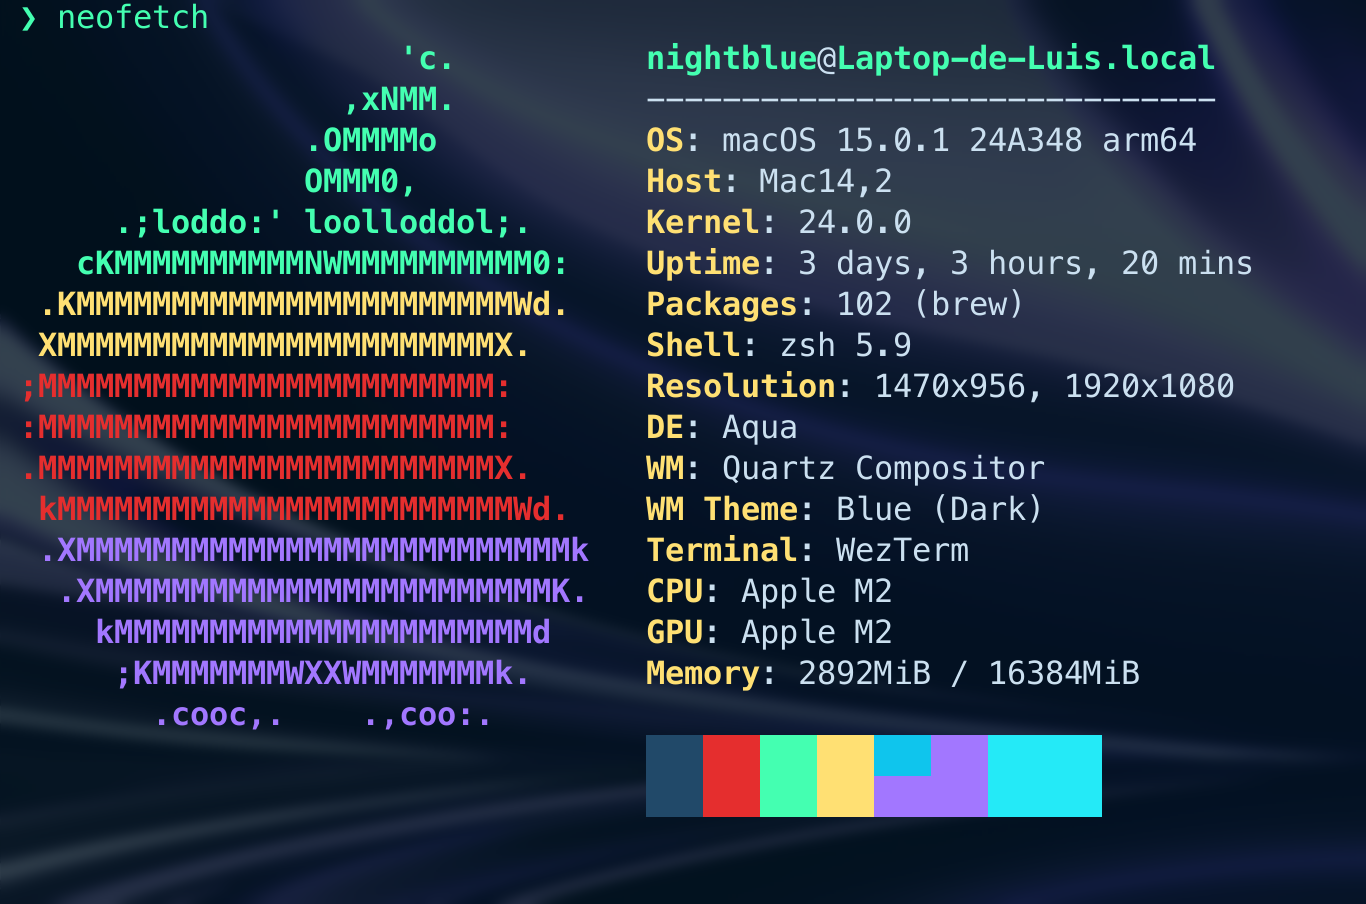
\includegraphics[width=0.9\textwidth]{images/neofetch.png}